\setcounter{section}{24}

\section{Конечные цепные дроби. Каноническая запись. Подходящие дроби. Рекуррентные соотношения для
числителей и знаменателей подходящих дробей (б/д). Следствия: несократимость подходящих дробей,
возрастание подходящих дробей с четными номерами и убывание подходящих дробей с нечетными
номерами.}
\textbf{Опр}\textit{ Конечной цепной дробью} называется выражение вида
\\
\\
$[a_0; a_1, a_2, ..., a_n] = a_0 +\frac{1}{ a_1 + \frac{1}{\ddots + \frac{1}{a_n}}}$, где $a_0 \in Z, a_i \in N \ \forall i >=1$\\
$a_i - $\textit{элементы цепной дроби, или неполные частные}
\\
Каноническая запись цепной дроби определяется индуктивно:\\
\begin{itemize}
    \item[1] $[a_0] = \frac{a_0}{1}$
    \item[2] Пусть для всех дробей с n элементами каноническая запись определена
    \item[3] $[a_0; a_1, ..., a_n] = a_0 + \frac{1}{[a_1; a_2, ..., a_n]} = a_0 + \frac{1}{p/q} = \frac{pa_0 + q}{p}$ 
\end{itemize}
\textbf{Опр}\\ $[a_0; a_1, ..., a_k] = \frac{p_k}{q_k}$ - k-ая подходящая дробь
\\
\\
\textbf{Теорема}\\
$p_{k+2} = a_{k+2}p_{k+1} + p_k \\ q_{k+2} = a_{k+2}q_{k+1} + q_k$
\\

\textbf{Следствие 1}
\begin{itemize}
\item[1] $\frac{p_{k+2}}{q_{k+2}} - \frac{p_{k+1}}{q_{k+1}} = \frac{(-1)^{k+1}}{q_{k+1}q_{k+2}}$
    \item [2] Kаноническая запись цепной дроби является несократимой
\end{itemize}

$\blacktriangle$
\\
$p_{k+2} - p_k = a_{k+2}p_{k+1}, \  q_{k+2} - q_k = a_{k+2}q_{k+1} \\ \\ \frac{p_{k+2} - p_k}{q_{k+2} - q_k} = \frac{a_{k+2}p_{k+1}}{a_{k+2}q_{k+1}} \\ \\ {p_{k+2}q_{k+1} - p_k q_{k+1}} = p_{k+1}q_{k+2} -  p_{k+1}q_k
\\ \\ $
Обозначим ЛЧ $b(k+2)$, ПЧ -$b(k+1)\\ b(1) = p_1 q_0 - q_1 p_0 = (a_0 a_1 + 1) * 1 - a_1 a_0 = 1\\ \\  p_{k+2}q_{k+1} - q_{k+2}p_{k+1} = (-1)^{k+1} \Longrightarrow \frac{p_{k+2}}{q_{k+2}} - \frac{p_{k+1}}{q_{k+1}} = \frac{(-1)^{k+1}}{q_{k+1} q_{k+2}}\\ \\$ 
Предположим, что каноническая запись цепной дроби сократима. Тогда $\frac{p_{k+2}}{q_{k+2}}$ - сократима, тогда $\exists \ d:\  p_{k+2}, q_{k+2} \  \vdots \ d \Longrightarrow p_{k+2}q_{k+1} - q_{k+2}p_{k+1} \ \vdots \ d$. Противоречие$ \\ \ \ \blacksquare$
\\
\\
\textbf{Замечание}\\
Из этого утверждения следует, что подходящие дроби с четными номерами меньше, чем с нечетными
\\
\\
\textbf{Следствие 2}\\
Подходящие дроби с четными номерами возрастают, с нечетными - убывают
\\$\blacktriangle$
\\
$p_{k+2} = a_{k+2}p_{k+1} + p_k *q_{k}\\ q_{k+2} = a_{k+2}q_{k+1} + q_k * p_k\\ \\ p_{k+2}q_k = a_{k+2}p_{k+1}q_{k} + p_k q_k \\ q_{k+2} p_k = a_{k+2}q_{k+1}p_k + q_k p_k \\ \\ p_{k+2}q_k - q_{k+2}p_k = a_{k+2}(p_{k+1}q_k - q_{k+1}p_k) = a_{k+2} (-1)^{k} \\ \\ \frac{p_{k+2}}{q_{k+2}} - \frac{p_k}{q_k} = \frac{a_{k+2} *(-1)^k}{q_k q_{k+2}}$
\\При четном k правая часть положительна, при нечетном - отрицательна
\\
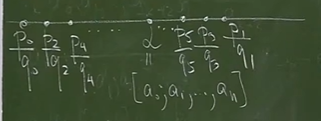
\includegraphics[width = 10cm]{images/25}
$\blacksquare$


\section{Рекуррентные соотношения для числителей и знаменателей подходящих дробей (доказательство).}
$\blacktriangle$  Будем доказывать по индукции
\begin{itemize}
    \item[1] База: k = 0; $[a_0] = \frac{a_0}{1} = \frac{p_0}{q_0}, [a_0; a_1] = a_0 + \frac{1}{a_1} = \frac{a_0 a_1 + 1}{a_1} = \frac{p_1}{q_1}, [a_0; a_1, a_2] = a_0 + \frac{1}{a_1 + \frac{1}{a_2}} = a_0 + \frac{a_2}{a_1a_2 + 1} = \frac{a_0a_1a_2 + a_0 + a_2}{a_1 a_2} = \frac{p_2}{q_2}\\ \\ a_0a_1a_2 + a_0 + a_2 = a_2a_0a_1 + a_2 + a_0 = a_2 * p_1 + p_0 \Longrightarrow$ Сошлось! Ура!
    \item[2] $a_0 + \frac{1}{[a_1; a_2,..., a_{k+2}]} = [a_0; a_1,..., a_{k+2}] = \frac{p_{k+2}}{q_{k+2}}$\\ Положим $[a_1; a_2, ..., a_i] = \frac{p_{i}'}{q_i'}$. Тогда $\frac{p_{k+2}}{q_{k+2}} = a_0 +  \frac{p_{k+2}'}{q_{k+2}'} = \frac{a_0p_{k+2}' + q_{k+2}'}{p_{k+2}'} \\ \\ p_{k+2}' = a_{k+2}p_{k+1}' + p_k', \ q_{k+2}' = a_{k+2}q_{k+1}' + q_k'$
    \\
    \\
    $\frac{p_{k+2}}{q_{k+2}} = \frac{a_0 a_{k+2} p_{k+1}' + a_0 p_k' + a_{k+2}q_{k+1}' + q_k'}{a_{k+2}p_{k+1}' + p_k'} = \frac{a_{k+2}(a_0 p_{k+1}' + q_{k+1}') + a_0 p_k' + q_k'}{a_{k+2}p_{k+1}' + p_k'}$ \\ \\ Теперь заметим, что $\frac{p_{k+2}}{q_{k+2}} = \frac{a_0p_{k+2}' + q_{k+2}'}{p_{k+2}'} \Longrightarrow p_i = a_0 p_i' + q_i', \ q_i = p_i' \Longrightarrow  \frac{a_{k+2}(a_0 p_{k+1}' + q_{k+1}') + a_0 p_k' + q_k'}{a_{k+2}p_{k+1}' + p_k'} = \frac{a_{k+2} p_{k+1} + p_{k}}{a_{k+2}q_{k+1} + q_k} \ \blacksquare$
\end{itemize} 


\section{Определение бесконечной цепной дроби. Доказательство сходимости соответствующих подходящих
цепных дробей (можно пользоваться без доказательства соотношениями на их коэффициенты).}
\textbf{Опр} \textit{Бесконечной цепной дробью} называется выражение вида:\\  $[a_0; a_1, a_2, ...] = a_0 +\frac{1}{ a_1 + \frac{1}{a_2 + \frac{1}{\ddots}}}$, где $a_0 \in Z, a_i \in N \ \forall i >=1$
\\
\textbf{Опр} \textit{Величиной бесконечной цепной дроби} называется предел её подходящих дробей, то есть такое число $\alpha = \underset{n->\infty}{lim}\frac{P_n}{Q_n}$\\ \\
\textbf{Теорема}
\\
Соответствующие подходящие цепные дроби сходятся. $\ \exists \underset{n->\infty}{lim}\frac{P_n}{Q_n} \\ \blacktriangle$ 
Согласно следствиям 1 и 2 из Теоремы о рекуррентных соотношениях для числителей и знаменятелей подходящих дробей последовательность дробей с четными номерами возрастает и ограничена сверху, а последовательность с нечетными номерами ограничена снизу и убывает, значит, обе эти последовательности имеют предел. $|\frac{P_n}{Q_n} - \frac{P_{n+1}}{Q_{n+1}}| = \frac{1}{Q_n Q_{n+1}}$
\\ В силу того, что $Q_{n+2} = a_{n+2}Q_{n+1} + Q_n, \  Q_{n+2} \geq Q_n \Longrightarrow \frac{1}{Q_n Q_{n+1}} \longrightarrow 0 \Longrightarrow |\frac{P_n}{Q_n} - \frac{P_{n+1}}{Q_{n+1}}|  \longrightarrow 0 \Longrightarrow$ пределы последовательностей совпадают, тогда и $\frac{P_n}{Q_n}$ сходится $\blacksquare$


\section{Бесконечные периодические цепные дроби. Теорема о периодичности дроби для квадратичной иррациональности (доказательство в одну сторону). Умение находить периодическую цепную дробь по её значению, и наоборот, нахождение значения дроби по её периоду.}
\textbf{Опр} Бесконечная цепная дробь вида

$[a_0; a_1, . . . , a_k, a_{k+1}, . . . , a_{k+T} , a_{k+1}, . . . , a_{k+T} , . . .] = [a_0; a_1, . . . , a_k, \overline{a_{k+1}, . . . , a_{k+T}}]$ называется \textit{периодической} с периодом $a_{k+1}, . . . , a_{k+T}$ . Набор $a_0, a_1, . . . , a_k$ называется \textit{предпериодом}.
\\
\\
\textbf{Опр} Иррациональное число $\alpha$ называется \textit{квадратичной иррациональностью}, если $\alpha$ - корень квадратного уравнения с целыми коэффициентами.
\\
\\
\textbf{Теорема}\\
Если $\alpha = [a_0; a_1, . . . , a_k, \overline{a_{k+1}, . . . , a_{n}}]$, то $\alpha$ - квадратичная иррациональность
\\
$\blacktriangle \ \beta = [\overline{a_{k+1}; a_{k+2}, ...,  a_n}] = a_{k+1} + \frac{1}{\ddots + a_n + \frac{1}{[\overline{a_{k+1}; a_{k+2}, ...,  a_n}] = \beta}}$
\\
\\
$\frac{a_n\beta + 1}{\beta}; \ \frac{\beta}{a_n \beta + 1} + a_{n-1} = \frac{\beta + a_{n-1}a_n\beta + a_{n-1}}{a_n\beta + 1}$\\
Заметим, что раскрывая таким образом мы получаем дробь вида $\frac{c\beta + d}{c'\beta + d'} = \beta$
\\
\\
$a_{0} + \frac{1}{\ddots + a_k + \frac{1}{\beta}}$
\\
Заметим две прекрасные вещи: \\
Если $\beta$ - решение квадратного уравнения, то $\frac{1}{\beta}$ - тоже является решением квадратного уравнения $\Longrightarrow \frac{1}{\beta}$ -  также квадратичная иррациональность. (Достаточно поделить уравнение для $\beta$ на $x^2$)
\\
Если $\beta$ - решение квадратного уравнения, то $\forall \gamma \in N \ \beta + \gamma \ -$ решение квадратного уравнения, т.е. квадратичная иррациональность. ( Если $c_2x^2 + c_1 x + c_0 = 0$ -  уравнение с корнем $\beta$, то $c_2(x - \gamma)^2 + c_1 (x - \gamma) + c_0 = 0$ - уравнение с корнем $\beta + \gamma$).
\\
Пользуясь тем, что прибавление к квадратичной иррациональности натурального числа и обратное к квадратичной иррациональности - квадратичная иррациональность, получаем, что $\alpha$ - квадратичная иррациональность $\ \blacksquare$

\subsection*{Нахождение периодической цепной дроби по её значению, и нахождение значения дроби по её периоду}
Пусть дана периодическая цепная дробь $[5; \overline{1, 2, 1 ,10}] = a$. Найти ее значение\\
Алгоритм: \\
1. Выделяем часть с периодом: $[\overline{1; 2, 1 ,10}] = x$ \\
2. Расписываем дробь, пока не дойдем до первого периода, приравниваем цепную дробь в знаменателе к x, всю дробь приравниваем к x:
$x = 1 +\frac{1}{2 + \frac{1}{1 + \frac{1}{10 + \frac{1}{\overline{[1; 2, 1 ,10]}}}}} = 1 +\frac{1}{2 + \frac{1}{1 + \frac{1}{10 + \frac{1}{x}}}}$\\
3. Начинаем переворчивать: $x = 1 +\frac{1}{2 + \frac{1}{1 + \frac{x}{10x + 1}}} = 1 +\frac{1}{2 + \frac{10x + 1}{11x + 1}} =  1 +\frac{11x + 1}{32x + 3} = \frac{43x + 4}{32x + 3} \Longrightarrow 32x^2 - 40x - 4 = 0 \Longrightarrow x = \frac{\sqrt{33} + 5}{8} $\\
4. Находим а. $a = 5 + \frac{1}{x} = 5 + \frac{8}{\sqrt{33} + 5} = \frac{33 + 5\sqrt{33}}{\sqrt{33} + 5} $
\\
\\
Пусть дано значение $a = \sqrt{2}$. Найти цепную дробь\\
Алгоритм:
1. Выделяем целую часть: $1 + (\sqrt{2} - 1)$ \\
2. 2. Если число уже встречалось в разложении, мы нашли период. Ура! Иначе переворачиваем дробную часть: $1 + \frac{1}{ \frac{1}{\sqrt{2} - 1}}$\\
3. Домножаем на сопряженное:  $1 + \frac{1}{ \frac{\sqrt{2} + 1}{1}} = 1 + \frac{1}{\sqrt{2} + 1} $\\
4. Вернуться к шагу 1\\
Таким образом, получим:\\
$1 + \frac{1}{\sqrt{2} + 1} = 1 + \frac{1}{ 2 + (\sqrt{2} -1)}$\\
$\sqrt{2} -1$ уже встречалось, значит, дробь: $[1;\overline{2}]$